\chapter{Simulation Results and Discussion}
\thispagestyle{fancy}

\section{Fractals}
As discussed in section \ref{sec:CAandSOC}, in order to show that a dynamical system exhibits SOC, some fractal nature must be present. As done analytically for a 1-D-model in~\cite{fractal_avalanching}, we can plot the energy of a system over time according to the definition of normalized energy
\[
E(t) = \int_f h(x,y,t)^2 df
\]
where $h$ is the height of a site at position $(x,y)$ of the field $f$ at time $t$. In MATLAB/Octave, at the end of every main loop iteration the energy is calculated:
\begin{lstlisting}
ee(t) = sum(sum(f.^2));
\end{lstlisting}
As the energy series in 1-dimensional case shows fractal properties (see~\cite{fractal_avalanching}), the question arises if this is true for a 2-dimensional case.

\section{Power-law Distributions}

In this section, investigations of the avalanche size and lifetime distributions are shown according to different boundary conditions: periodic and open.


\subsection{Periodic Boundary Conditions}

For periodic boundary conditions, no grain gets lost as long as no friction is introduced. As a consequence, the driving time and the lattice shize need to be chosen carefully, in order not to run into a situation of a never-ending avalanche. Also, to analyze the distribution, good statistics must be present - a reasonably large lattice is needed. Although, theoretically, the lattice is of infinite size (due to its periodic nature), which implies that the size should not matter.

Here, a $100\times 100$ lattice is studied with a driving time $T=5000$. The results are presented in the figures~\ref{sp}. The power-law behaviour is easily recognizable for the avalanche size and for the avalanche lifetime, although the latter fit is of poorer quality.

\begin{figure} 
\begin{center}
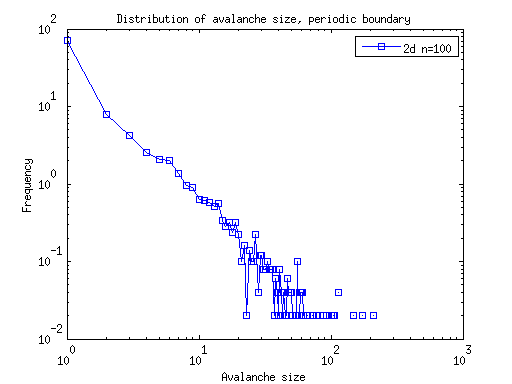
\includegraphics[width=0.75\textwidth]{results/sp.png} \\
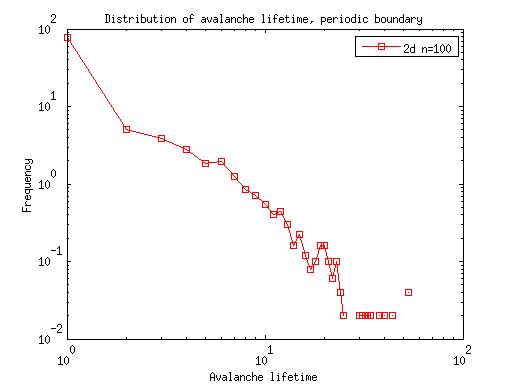
\includegraphics[width=0.75\textwidth]{results/tp.png} 
\caption{Avalanche size and lifetime distribution for a $100\times100$ lattice, with periodic boundary conditions. 
The driving time is $T=5000$.  }
\label{sp}
\end{center}
\end{figure} 

Higher dimensions are not treated here, due to high memory and simulation runtime requirements. As real systems are finite and dissipative, the periodic boundary case without grain loss is not of much intereset, i.e. it is not considered a SOC phenomenon. Instead, a friction parameter is introduced and discrete grain addition is replaced by a continuous one, thus replacing the integer field by a \emph{real} field and presenting a more realistic model.

The periodic boundary in principle implies lattice size independence, which will represent a computational advantage, as a small lattice can be chosen. However, the driving time will increase in order to get enough statistics.

Results of this situation for $d=2$, with $n=10$, $n=50$ and $n=100$ are shown in figures~\ref{spf1} and~\ref{spf2}. A clear cut-off for large avalanche number due to friction is seen, but with a nice power-law distribution for small avalanches. The lifetime is not shown, as it shows worse statistics, which do not differ much from the case in figure~\ref{sp}.



\begin{figure}
\begin{center}
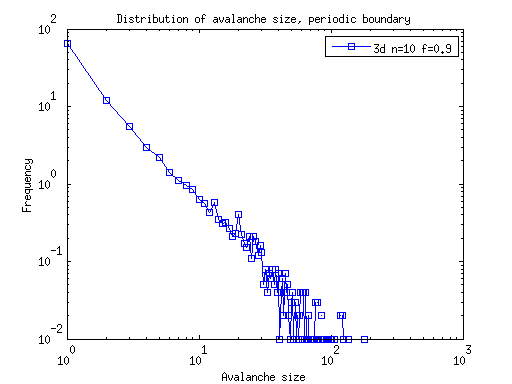
\includegraphics[width=0.75\textwidth]{results/3spf.png} \\
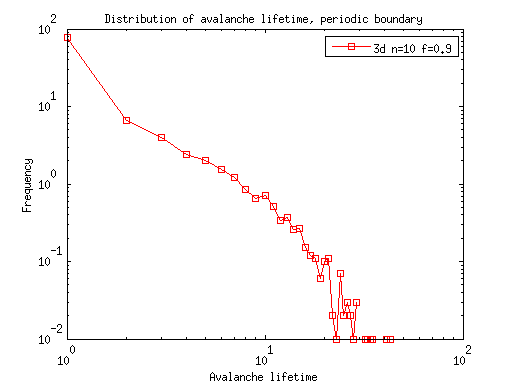
\includegraphics[width=0.75\textwidth]{results/3tpf.png} \\
\caption{Avalanche size and lifetime distribution for a $3d$ lattice with friction and periodic boundary conditions. }
\label{dspf3}
\end{center}
\end{figure}

\begin{figure}
\begin{center}
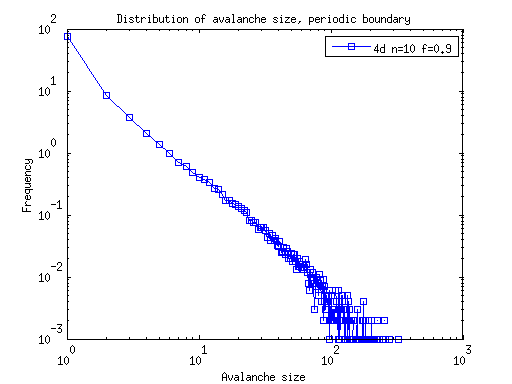
\includegraphics[width=0.75\textwidth]{results/4spf.png} \\
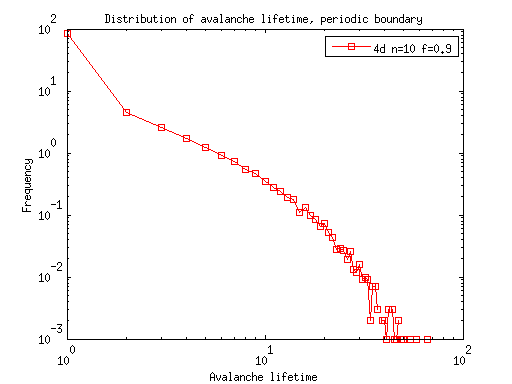
\includegraphics[width=0.75\textwidth]{results/4tpf.png} \\
\caption{Avalanche size and lifetime distribution for a $4d$ lattice with friction and periodic boundary conditions. }
\label{dspf4}
\end{center}
\end{figure}


\begin{figure}
\begin{center}
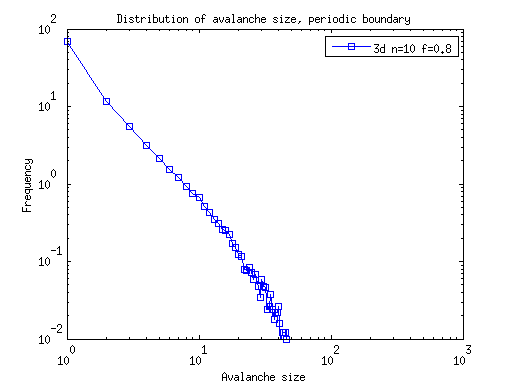
\includegraphics[width=0.75\textwidth]{results/3spf08.png}
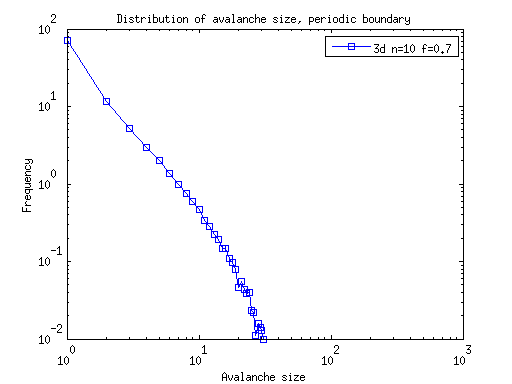
\includegraphics[width=0.75\textwidth]{results/3spf07.png}
\caption{Avalanche size distribution for a $3d$ lattice with different friction parameters using periodic boundary conditions. }
\label{3spf}
\end{center}
\end{figure}


\begin{figure}
\begin{center}
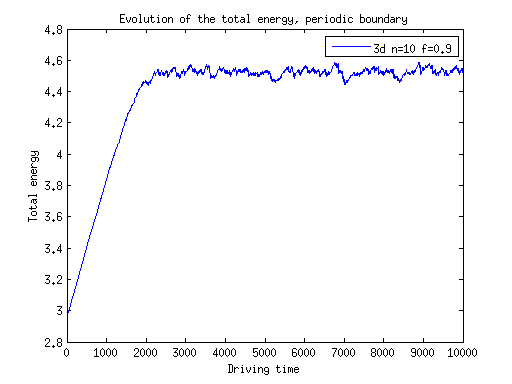
\includegraphics[width=0.75\textwidth]{results/3ep.png}
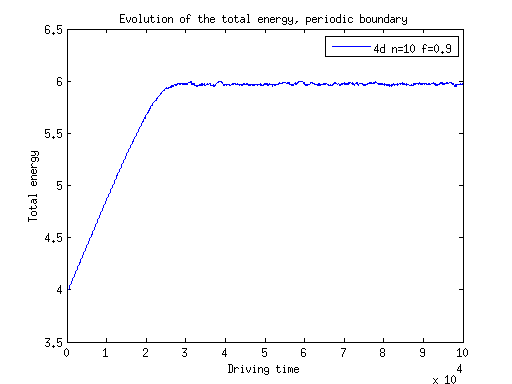
\includegraphics[width=0.75\textwidth]{results/4ep.png}
\caption{Normalized total energy evolution for $3d$ and $4d$ lattices with friction and periodic boundary conditions. }
\label{ep}
\end{center}
\end{figure}


\begin{figure}
\begin{center}
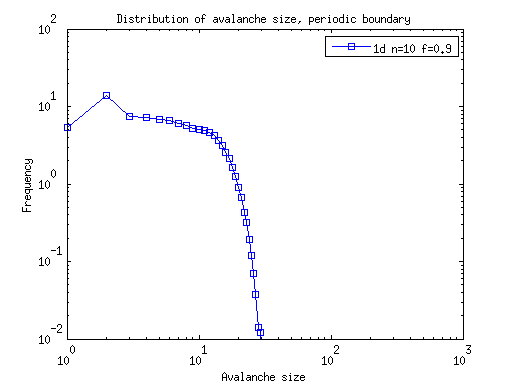
\includegraphics[width=0.75\textwidth]{results/1sp.png}
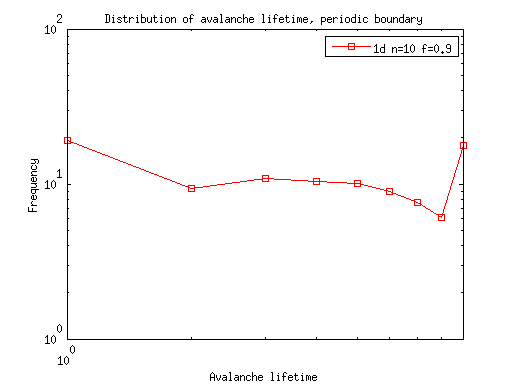
\includegraphics[width=0.75\textwidth]{results/1tp.png}
\caption{Avalanche size and lifetime distribution for $1d$ lattices with friction, periodic boundary conditions and $T=100 000$. There is no criticality for this case. }
\label{1p}
\end{center}
\end{figure} 



The importance of the dissipation becomes clear as the critical exponent changes for different values of friction.

From figures~\ref{spf1} and~\ref{spf2} we can conclude that small lattices can also be used with a small driving time, saving computational capacity. Therefore, this case will be used to explore higher dimensional lattices, that are computationally more costly. Figures~\ref{dspf3} and~\ref{dspf4} show the results of the $3d$ and the $4d$ case respectively. The cut-off effect due to friction is much less than for the $2d$ lattice. The effect of an increase in the friction value is shown in figure~\ref{3spf}. From this analysis, clearly, the dissipation plays an important role. Nevertheless, \emph{on average}, the total energy of lattice is kept constant when the system evolves (see figure~\ref{ep}). Furthermore, for $d=1$, no critical behaviour is seen, in agreement with the prediction of theory presented in~\cite{soc} (the situation for open boundary has also been checked to be the same). Refer to figure~\ref{1p} for the results.

\begin{figure} 
\begin{center}
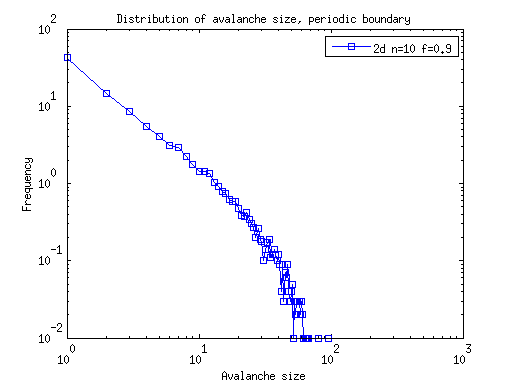
\includegraphics[width=0.75\textwidth]{results/spf.png}
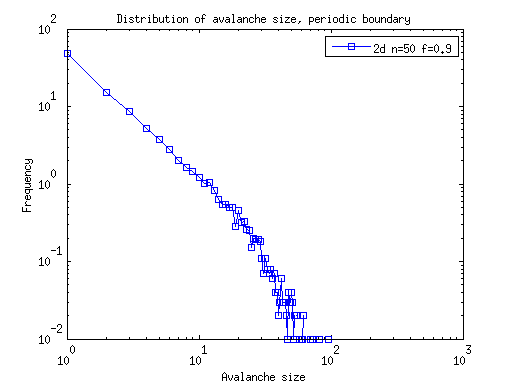
\includegraphics[width=0.75\textwidth]{results/spf50.png} \\
\caption{Avalanche size distribution for a $2d$ lattice with friction and periodic boundary conditions. The driving time is $T=10 000$ and the lattice size is $n=10$ and $n=50$, respectively. }
\label{spf1}
\end{center}
\end{figure}


\begin{figure} 
\begin{center}
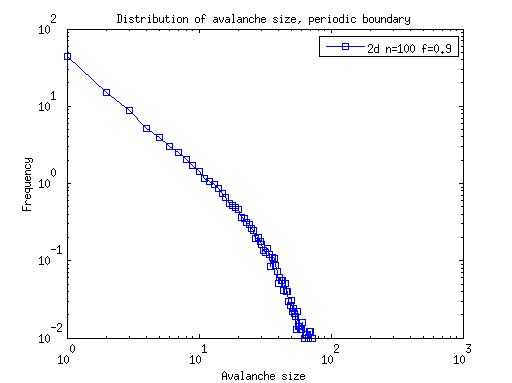
\includegraphics[width=0.75\textwidth]{results/spf100.png} 
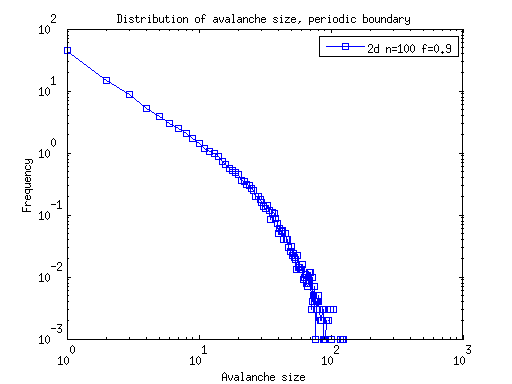
\includegraphics[width=0.75\textwidth]{results/spf100a.png}
\caption{Avalanche size distribution for a $2d$ lattice with friction and periodic boundary conditions. The driving time is $T=100 000$. The first plot is restricted in the $y$-direction for a good comparison with the $n=10$ and $n=50$ cases. The second one shows the complete statistics, where a cut-off due to friction is seen clearly. }
\label{spf2}
\end{center}
\end{figure} 




\subsection{Finite boundary conditions}

In the case of finite boundaries, grains drop automatically when boundary sites topple. However, unlike the previous case, finite size effects must be dealt with.

A perturbation in the boundary might cause a different avalanche distribution than a perturbation placed in the bulk. One might expect a bulk perturbation to produce bigger avalanches, as the grain has to be transported further in order to be lost at the boundaries.

Here, this effect is studied for 2-dimensional case and remarkably, different avalanche size distributions can be seen (figure~\ref{sv}). Furthermore, the high dispersion in large avalanche sizes for the bulk case causes a worse power-law fit compared to the boundary perturbation case.

For random perturbation sites, the result is closer to the bulk one than to the boundary one.

\begin{figure} 
\begin{center}
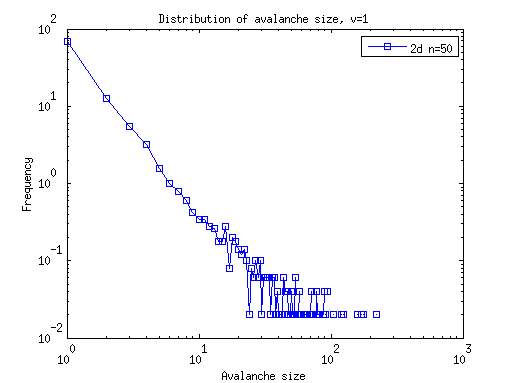
\includegraphics[width=0.75\textwidth]{results/sv1.png}
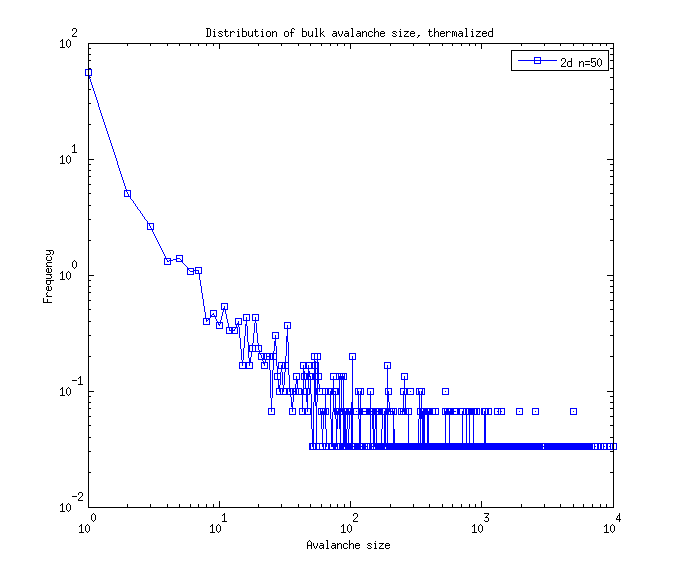
\includegraphics[width=0.75\textwidth]{results/sbulk_th.png} 
\caption{Avalanche size distribution for $50\times50$ lattice for different perturbation sites (first plot: site $(1,1)$, upper left the corner; second plot: bulk site, $(25,25)$). The driving time is $T=5000$.}
\label{sv}
\end{center}
\end{figure} 


The relation of the number of sites in the volume to the number of sites at boundary should be proportional to the lattice size $n$, as it is basically the ratio of volume and area. This implies that on a large lattice one encounters more large avalanches than on a smaller lattice. See figure~\ref{sn}.

\begin{figure}
\begin{center}
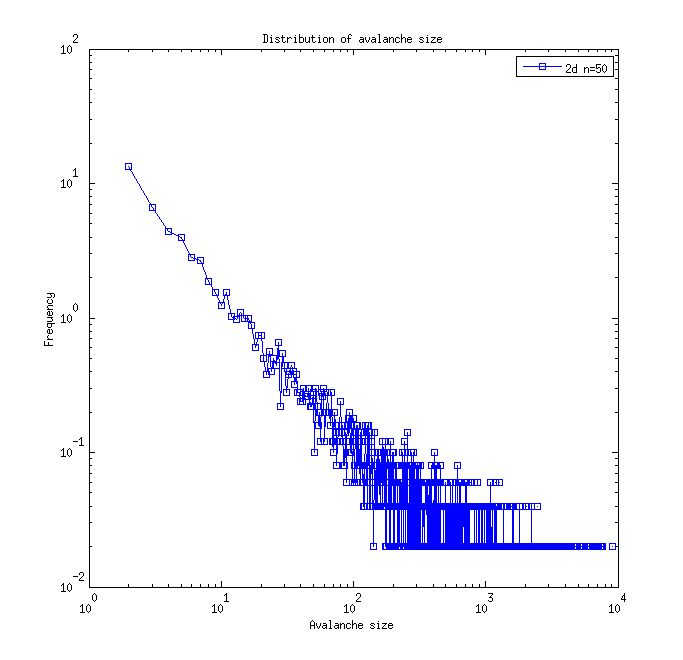
\includegraphics[width=0.75\textwidth]{results/2sn50.png}
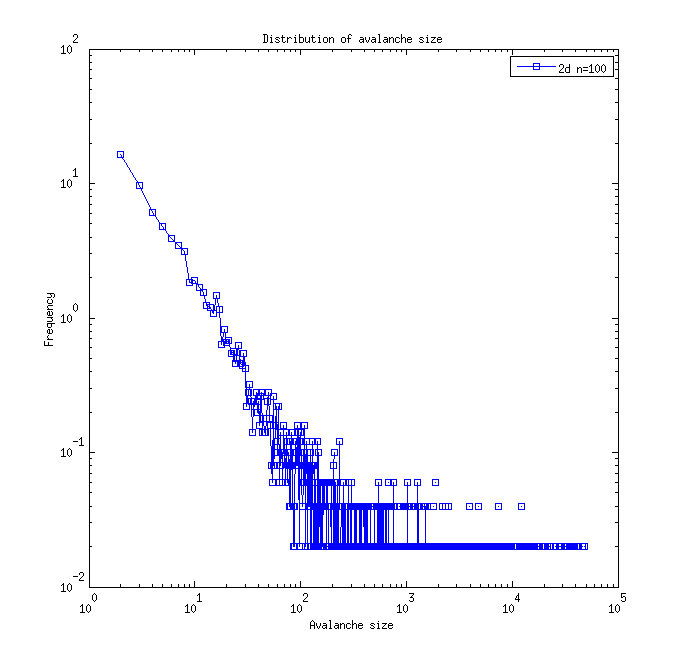
\includegraphics[width=0.75\textwidth]{results/2sn100.png}
\caption{Avalanche size distribution for $2d$ lattices with different sizes and open boundary conditions.}
\label{sn}
\end{center}
\end{figure} 

Adding friction (and thus going to a more realistic case), the number of large avalanches reduces. Again, friction is cruxial for generating a power-law like distribution and for the cut-off effect discussed before.

\begin{figure}
\begin{center}
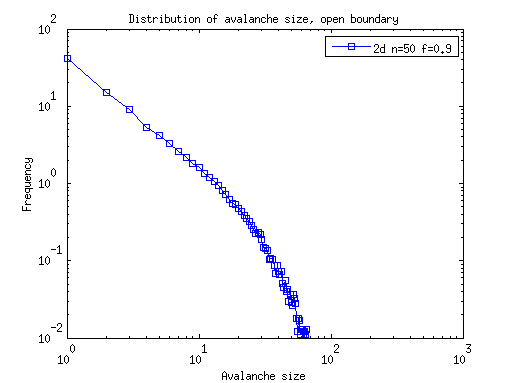
\includegraphics[width=0.75\textwidth]{results/2sof.png}
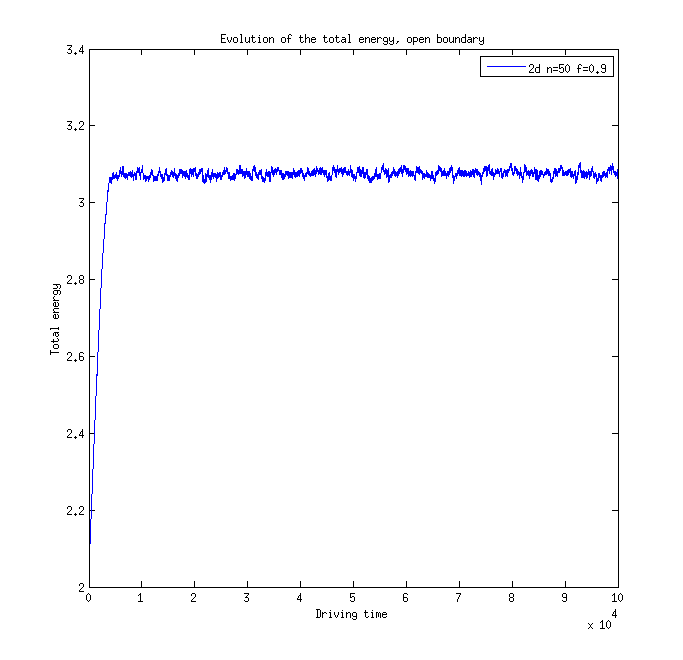
\includegraphics[width=0.75\textwidth]{results/2eof.png}
\caption{Avalanche size distribution and energy evolution for a $2d$ lattice with friction and open boundary conditions.}
\label{so}
\end{center}
\end{figure} 

\subsection{Slowly Driven Test}
Apart from friction, additional grain addition during the avalanche process can be studied. For this, a probability $h$ of an additional grain placement during an avalanche is introduced. The results in figure~\ref{soh} show that the system indeed fits less into a power-law curve. The relative amount of large avalanches rises, as there is a probability of a new avalanche to happen during another one and these two would be counted as one, but a bigger one.

In \emph{mean field theory}, one can consider this $h$ parameter as a fine-tuning parameter, as when $h\longrightarrow0$, the systems turns to exhibit more power-law behaviour.

\begin{figure}
\begin{center}
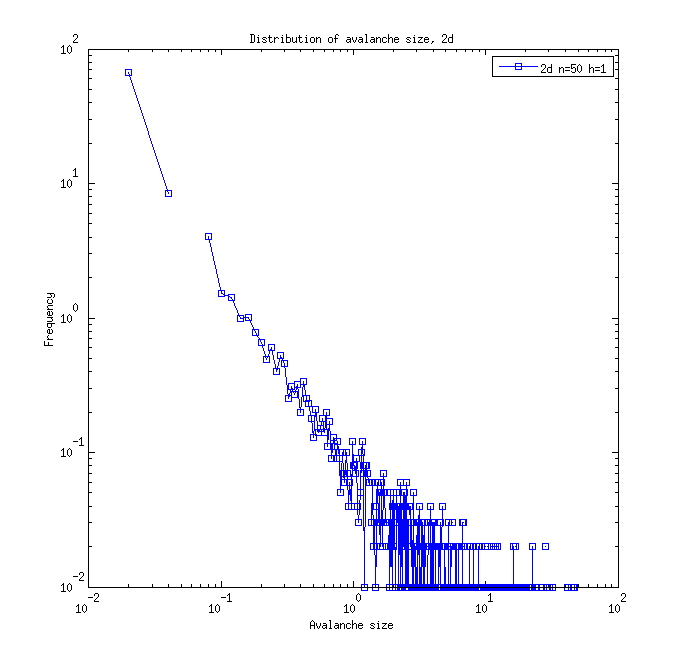
\includegraphics[width=0.75\textwidth]{results/2soh.png}
\caption{Avalanche size distribution for a $2d$ lattice with open boundary conditions and $h=1$. }
\label{soh}
\end{center}
\end{figure} 

From this analysis, we see that it is important that dissipation exists during the avalanche time, rather losing energy in the boundary or by energy dissipation during the propagation. (???)

During the driving time the energy of the system, defined as the sum of the values of the field of all sites, tends to oscillate around a constant value. Each additional grain is compensated with the dissipation during avalanche. For examples see figures~\ref{so} and~\ref{ep}.


